

\tikzset{every picture/.style={line width=0.75pt}} %set default line width to 0.75pt        

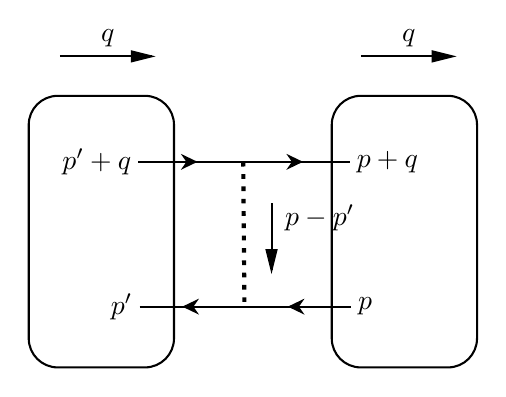
\begin{tikzpicture}[x=0.75pt,y=0.75pt,yscale=-1,xscale=1]
%uncomment if require: \path (0,300); %set diagram left start at 0, and has height of 300

%Straight Lines [id:da9979613690985549] 
\draw [color={rgb, 255:red, 0; green, 0; blue, 0 }  ,draw opacity=1 ][line width=0.75]    (191.89,155.8) -- (242.35,155.8) ;
\draw [shift={(220.32,155.8)}, rotate = 180] [fill={rgb, 255:red, 0; green, 0; blue, 0 }  ,fill opacity=1 ][line width=0.08]  [draw opacity=0] (8.04,-3.86) -- (0,0) -- (8.04,3.86) -- (5.34,0) -- cycle    ;
%Straight Lines [id:da5231803030380069] 
\draw [color={rgb, 255:red, 0; green, 0; blue, 0 }  ,draw opacity=1 ][line width=0.75]    (242.35,155.8) -- (293.58,155.8) ;
\draw [shift={(271.16,155.8)}, rotate = 180] [fill={rgb, 255:red, 0; green, 0; blue, 0 }  ,fill opacity=1 ][line width=0.08]  [draw opacity=0] (8.04,-3.86) -- (0,0) -- (8.04,3.86) -- (5.34,0) -- cycle    ;
%Straight Lines [id:da4079322973600161] 
\draw [color={rgb, 255:red, 0; green, 0; blue, 0 }  ,draw opacity=1 ][line width=0.75]    (192.48,225.57) -- (242.94,225.57) ;
\draw [shift={(213.01,225.57)}, rotate = 0] [fill={rgb, 255:red, 0; green, 0; blue, 0 }  ,fill opacity=1 ][line width=0.08]  [draw opacity=0] (8.04,-3.86) -- (0,0) -- (8.04,3.86) -- (5.34,0) -- cycle    ;
%Straight Lines [id:da9026612092672825] 
\draw [color={rgb, 255:red, 0; green, 0; blue, 0 }  ,draw opacity=1 ][line width=0.75]    (242.94,225.57) -- (294.17,225.57) ;
\draw [shift={(263.85,225.57)}, rotate = 0] [fill={rgb, 255:red, 0; green, 0; blue, 0 }  ,fill opacity=1 ][line width=0.08]  [draw opacity=0] (8.04,-3.86) -- (0,0) -- (8.04,3.86) -- (5.34,0) -- cycle    ;
%Straight Lines [id:da7016774699366952] 
\draw [line width=1.5]  [dash pattern={on 1.69pt off 2.76pt}]  (242.35,155.8) -- (242.94,225.57) ;
%Rounded Rect [id:dp7248725342845543] 
\draw   (139,138) .. controls (139,130.27) and (145.27,124) .. (153,124) -- (195,124) .. controls (202.73,124) and (209,130.27) .. (209,138) -- (209,240.85) .. controls (209,248.59) and (202.73,254.85) .. (195,254.85) -- (153,254.85) .. controls (145.27,254.85) and (139,248.59) .. (139,240.85) -- cycle ;
%Straight Lines [id:da7227711421802434] 
\draw    (154,105) -- (198.17,105) ;
\draw [shift={(200.17,105)}, rotate = 180] [fill={rgb, 255:red, 0; green, 0; blue, 0 }  ][line width=0.08]  [draw opacity=0] (12,-3) -- (0,0) -- (12,3) -- cycle    ;
%Rounded Rect [id:dp10838249510257558] 
\draw   (285,138) .. controls (285,130.27) and (291.27,124) .. (299,124) -- (341,124) .. controls (348.73,124) and (355,130.27) .. (355,138) -- (355,240.85) .. controls (355,248.59) and (348.73,254.85) .. (341,254.85) -- (299,254.85) .. controls (291.27,254.85) and (285,248.59) .. (285,240.85) -- cycle ;
%Straight Lines [id:da6110642333116789] 
\draw    (299,105) -- (343.17,105) ;
\draw [shift={(345.17,105)}, rotate = 180] [fill={rgb, 255:red, 0; green, 0; blue, 0 }  ][line width=0.08]  [draw opacity=0] (12,-3) -- (0,0) -- (12,3) -- cycle    ;
%Straight Lines [id:da09763037399523022] 
\draw    (256,175.85) -- (256,207.85) ;
\draw [shift={(256,209.85)}, rotate = 270] [fill={rgb, 255:red, 0; green, 0; blue, 0 }  ][line width=0.08]  [draw opacity=0] (12,-3) -- (0,0) -- (12,3) -- cycle    ;

% Text Node
\draw (189.89,155.8) node [anchor=east] [inner sep=0.75pt]    {$\boldsymbol{p}' +\boldsymbol{q}$};
% Text Node
\draw (295.58,155.8) node [anchor=west] [inner sep=0.75pt]    {$\boldsymbol{p} +\boldsymbol{q}$};
% Text Node
\draw (190.48,225.57) node [anchor=east] [inner sep=0.75pt]    {$\boldsymbol{p}'$};
% Text Node
\draw (296.17,225.57) node [anchor=west] [inner sep=0.75pt]    {$\boldsymbol{p}$};
% Text Node
\draw (177.08,102) node [anchor=south] [inner sep=0.75pt]    {$\boldsymbol{q}$};
% Text Node
\draw (322.08,102) node [anchor=south] [inner sep=0.75pt]    {$\boldsymbol{q}$};
% Text Node
\draw (261,182.85) node [anchor=west] [inner sep=0.75pt]    {$\boldsymbol{p} -\boldsymbol{p}'$};


\end{tikzpicture}
